\section{oosalizer/parser.c-Dateireferenz}
\label{parser_8c}\index{oosalizer/parser.c@{oosalizer/parser.c}}
{\tt \#include $<$time.h$>$}\par
{\tt \#include $<$stdio.h$>$}\par
{\tt \#include $<$stdlib.h$>$}\par
{\tt \#include $<$string.h$>$}\par
{\tt \#include $<$unistd.h$>$}\par
{\tt \#include $<$ctype.h$>$}\par
{\tt \#include $<$sys/utsname.h$>$}\par
{\tt \#include $<$sys/times.h$>$}\par
{\tt \#include $<$sys/types.h$>$}\par
{\tt \#include \char`\"{}webalizer.h\char`\"{}}\par
{\tt \#include \char`\"{}lang.h\char`\"{}}\par
{\tt \#include \char`\"{}parser.h\char`\"{}}\par


Include-Abh\"{a}ngigkeitsdiagramm f\"{u}r parser.c:\begin{figure}[H]
\begin{center}
\leavevmode
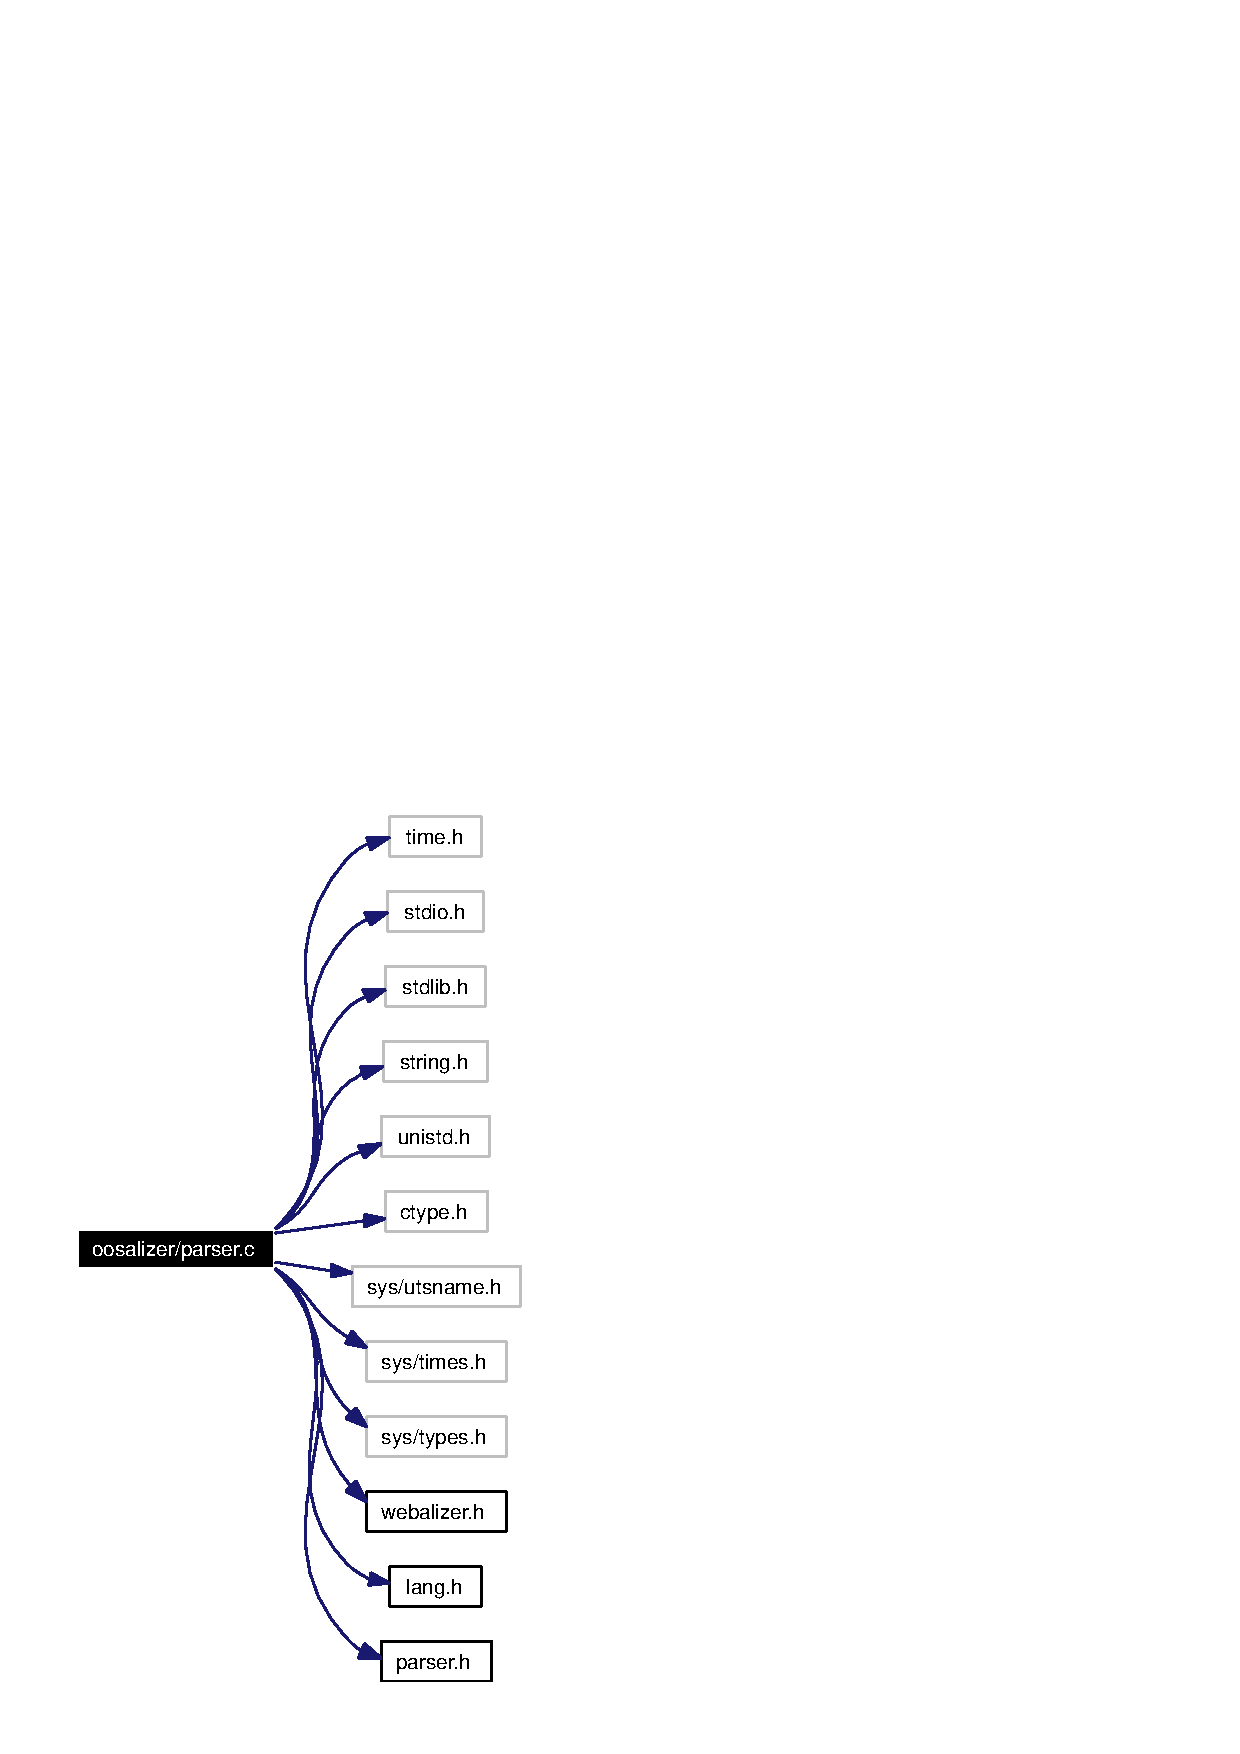
\includegraphics[width=125pt]{parser_8c__incl}
\end{center}
\end{figure}
\subsection*{Makrodefinitionen}
\begin{CompactItemize}
\item 
\#define {\bf CLK\_\-TCK}~\_\-SC\_\-CLK\_\-TCK
\end{CompactItemize}
\subsection*{Funktionen}
\begin{CompactItemize}
\item 
void {\bf fmt\_\-logrec} (char $\ast$)
\item 
int {\bf parse\_\-record\_\-web} (char $\ast$)
\item 
int {\bf parse\_\-record\_\-ftp} (char $\ast$)
\item 
int {\bf parse\_\-record\_\-squid} (char $\ast$)
\item 
int {\bf parse\_\-record} (char $\ast${\bf buffer})
\end{CompactItemize}


\subsection{Makro-Dokumentation}
\index{parser.c@{parser.c}!CLK_TCK@{CLK\_\-TCK}}
\index{CLK_TCK@{CLK\_\-TCK}!parser.c@{parser.c}}
\subsubsection{\setlength{\rightskip}{0pt plus 5cm}\#define CLK\_\-TCK~\_\-SC\_\-CLK\_\-TCK}\label{parser_8c_03df76d1f70664d745ca8de2864e39b3}




Definiert in Zeile 59 der Datei parser.c.

\subsection{Dokumentation der Funktionen}
\index{parser.c@{parser.c}!fmt_logrec@{fmt\_\-logrec}}
\index{fmt_logrec@{fmt\_\-logrec}!parser.c@{parser.c}}
\subsubsection{\setlength{\rightskip}{0pt plus 5cm}void fmt\_\-logrec (char $\ast$)}\label{parser_8c_05c2b956fa80dba2cd2fcce536158855}




Definiert in Zeile 76 der Datei parser.c.

Wird benutzt von parse\_\-record\_\-ftp(), parse\_\-record\_\-squid() und parse\_\-record\_\-web().\index{parser.c@{parser.c}!parse_record@{parse\_\-record}}
\index{parse_record@{parse\_\-record}!parser.c@{parser.c}}
\subsubsection{\setlength{\rightskip}{0pt plus 5cm}int parse\_\-record (char $\ast$ {\em buffer})}\label{parser_8c_f7f838e64a0d2b296d0b8b09b49d6b85}




Definiert in Zeile 101 der Datei parser.c.

Benutzt LOG\_\-CLF, LOG\_\-FTP, log\_\-rec, LOG\_\-SQUID, log\_\-type, parse\_\-record\_\-ftp(), parse\_\-record\_\-squid() und parse\_\-record\_\-web().\index{parser.c@{parser.c}!parse_record_ftp@{parse\_\-record\_\-ftp}}
\index{parse_record_ftp@{parse\_\-record\_\-ftp}!parser.c@{parser.c}}
\subsubsection{\setlength{\rightskip}{0pt plus 5cm}int parse\_\-record\_\-ftp (char $\ast$)}\label{parser_8c_630c3ac0dab48c2fba68649da4bb871e}




Definiert in Zeile 134 der Datei parser.c.

Benutzt log\_\-struct::datetime, fmt\_\-logrec(), log\_\-struct::hostname, log\_\-struct::ident, log\_\-rec, MAXHOST, MAXURL, log\_\-struct::resp\_\-code, log\_\-struct::url und log\_\-struct::xfer\_\-size.

Wird benutzt von parse\_\-record().\index{parser.c@{parser.c}!parse_record_squid@{parse\_\-record\_\-squid}}
\index{parse_record_squid@{parse\_\-record\_\-squid}!parser.c@{parser.c}}
\subsubsection{\setlength{\rightskip}{0pt plus 5cm}int parse\_\-record\_\-squid (char $\ast$)}\label{parser_8c_2b00ce99cc8f1387d75aeb7193968b21}




Definiert in Zeile 379 der Datei parser.c.

Benutzt log\_\-struct::datetime, debug\_\-mode, fmt\_\-logrec(), log\_\-struct::hostname, log\_\-struct::ident, log\_\-rec, MAXHOST, MAXIDENT, MAXURL, msg\_\-big\_\-host, msg\_\-big\_\-req, log\_\-struct::resp\_\-code, log\_\-struct::url, verbose und log\_\-struct::xfer\_\-size.

Wird benutzt von parse\_\-record().\index{parser.c@{parser.c}!parse_record_web@{parse\_\-record\_\-web}}
\index{parse_record_web@{parse\_\-record\_\-web}!parser.c@{parser.c}}
\subsubsection{\setlength{\rightskip}{0pt plus 5cm}int parse\_\-record\_\-web (char $\ast$)}\label{parser_8c_f79ff394bf86e83cffbcb560096f5052}




Definiert in Zeile 220 der Datei parser.c.

Benutzt log\_\-struct::agent, log\_\-struct::datetime, debug\_\-mode, fmt\_\-logrec(), log\_\-struct::hostname, log\_\-struct::ident, log\_\-rec, MAXAGENT, MAXHOST, MAXIDENT, MAXREF, MAXURL, msg\_\-big\_\-date, msg\_\-big\_\-host, msg\_\-big\_\-ref, msg\_\-big\_\-req, msg\_\-big\_\-user, log\_\-struct::refer, log\_\-struct::resp\_\-code, log\_\-struct::url, verbose und log\_\-struct::xfer\_\-size.

Wird benutzt von parse\_\-record().